\section{Lecture 8 | Integrating Learning and Planning}
Learn the model of the environment from the experience of the environment, and use planning to construct
a value function or policy. Also discuss about integrating and planning into a single architecture.

\subsubsection*{Model based and Model free RL}
\begin{itemize}
    \item Model based RL: Learn the model of the environment from the experience of the environment, and use planning to construct
    a value function or policy.
    \item Model free RL: Learn the value function or policy directly from the experience of the environment.
\end{itemize}

\subsection{Model based Reinforcement Learning}
\begin{figure}[H]
    \begin{minipage}{0.5\textwidth}
        \begin{itemize}
            \item \textbf{Advantages:}
            \begin{itemize}
                \item Can efficiently learn model by supervised learning methods
                \item Can reason about model uncertainty
            \end{itemize}
            \item \textbf{Disadvantages:}
            \begin{itemize}
                \item Learning a model, and then planning in it invokes two sources of approximation error
            \end{itemize}
        \end{itemize}
    \end{minipage}%
    \begin{minipage}{0.5\textwidth}
      % Your image goes here
      \centering
      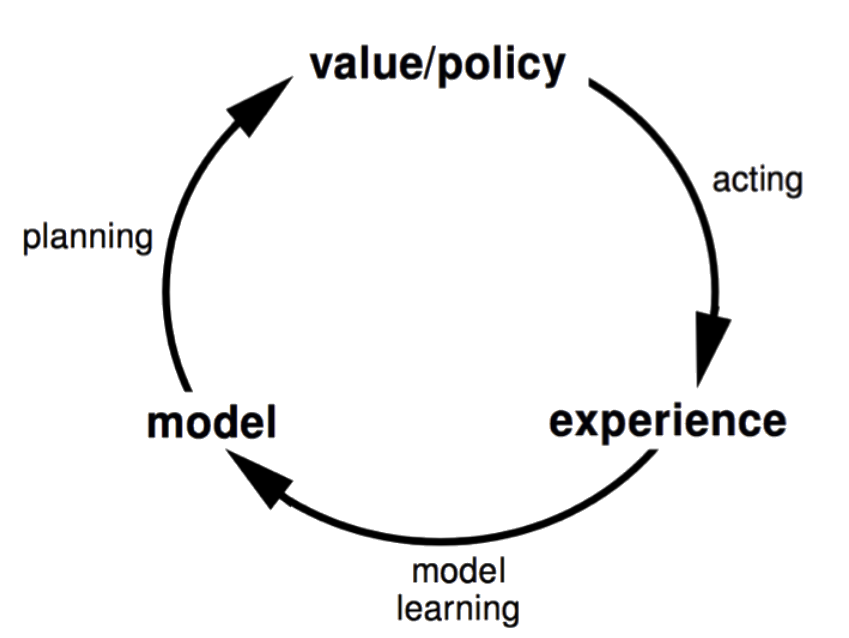
\includegraphics[height=0.5\textwidth]{figures/modelrlcycle.png}
      \caption{Model based RL cycle}
        \label{fig:modelrlcycle}
    \end{minipage}
\end{figure}
One of the clearlest example of model based RL is the game of chess. There are about \(10^{40}\) states in the
game of chess. In the game wven if we move from one state to another, the value function completly changes, i.e. the
value function is a very sharp. However the model of hte chess is simple, its just the rules of the game, and we can look
ahead and estimate the value function using tree search, in a much easier manner. 
So sometimes the model of the environment is much simpler and much useful than the value function or the policy.
\subsubsection{Learning a Model}
A model \(\mathcal{M}\) is a representaytion of an MDP \(\langle \mathcal{S}, \mathcal{A},
\mathcal{P}, \mathcal{R} \rangle\), parameterized by \(\eta\). Assuming that the state space
\(\mathcal{S}\) and action space \(\mathcal{A}\) are known, the model \(\mathcal{M} = \langle
\mathcal{P}_\eta, \mathcal{R}_\eta \rangle\) represents state transition 
\(\mathcal{P} _\eta \approx \mathcal{P}\) and reward function \(\mathcal{R}_\eta \approx
\mathcal{R}\). Thus,
\[
    \begin{aligned}
        S_{t+1} &\sim \mathcal{P}_\eta(S_{t+1}  | S_t, A_t) \\
        R_{t+1} &= \mathcal{R}_\eta(R_{t+1} | S_t, A_t)
    \end{aligned}        
\]
Typically we assume conditional independence between the state transitions and rewards, i.e.
\[
    \mathbb{P}\left[ S_{t+1}, R_{t+1} | S_t, A_t \right] = \mathbb{P}\left[ S_{t+1} | S_t, A_t \right]
\]

Thus, the goal is to model \(\mathcal{M} _\eta \) from experience \(\mathcal{D} = \{ S_1, A_1, R_2,
\ldots, S_T \}\). We can use supervised learning to learn the model:
\[
    \begin{aligned}
        S_1, A_1 &\rightarrow R_2, S_2 \\
        S_2, A_2 &\rightarrow R_3, S_3 \\
        \vdots & \\
        S_{T-1}, A_{T-1} &\rightarrow R_T, S_T
    \end{aligned}
\]
Learning \(s,a \to r\) is a regression problem, while learning \(s,a \to s'\) is a density estimation. SO 
using the supervised learning methods we can learn the model of the environment, i.e. pick a loss function say
mean squared error, KL divergence, etc. and then find the parameters of the model that minimizes the loss function.

\subsubsection*{Examples of Models}
\begin{itemize}
    \item Table Lookup Model
    \item Linear Expectation Model
    \item Linear Gaussian Model
    \item Gaussian Process Model
    \item Neural Network Model
    \item Deep Belief Network Model, etc.
\end{itemize}

\subsubsection{Tabule Lookup Model}
Mdoel is an explicyt MDP, \(\hat{\mathcal{P}}, \hat{\mathcal{R}}\). The main idea is simple, keep a count of
visits to each state action pair, and then use the counts to estimate the transition probabilities and the rewards.
\[
    \begin{aligned}
        \hat{\mathcal{P}}_{ss'}^a &= \frac{1}{N(s,a)} \sum_{t=1}^T \mathbb{I}(S_t = s, A_t = a, S_{t+1} = s') \\
        \hat{\mathcal{R}}_s^a &= \frac{1}{N(s,a)} \sum_{t=1}^T \mathbb{I}(S_t = s, A_t = a) R_{t+1}
    \end{aligned}  
\]
An alternative approach is to store everything. So at each time step record the expericence tuple
\[
    \langle S_t, A_t, R_{t+1}, S_{t+1} \rangle  
\]
and to to sample the model, randomly sample from the recorded experience, mathcing the
current state and action matching \(\langle s,a ,\cdot, \cdot \rangle\). 

\begin{example}[AB Example]
    Two states \(A\) and \(B\); no discounting; with 8 episodes of experience as:
    \begin{figure}[H]
        \begin{minipage}{0.5\textwidth}
          \[
            \begin{aligned}
                A, & 0, B, 0 \\
                B, & 1\\ 
                B, & 1\\        
                B, & 1\\        
                B, & 1\\        
                B, & 1\\        
                B, & 1\\        
                B, & 0\\        
            \end{aligned}
          \]
        \end{minipage}%
        \begin{minipage}{0.5\textwidth}
          % Your image goes here
          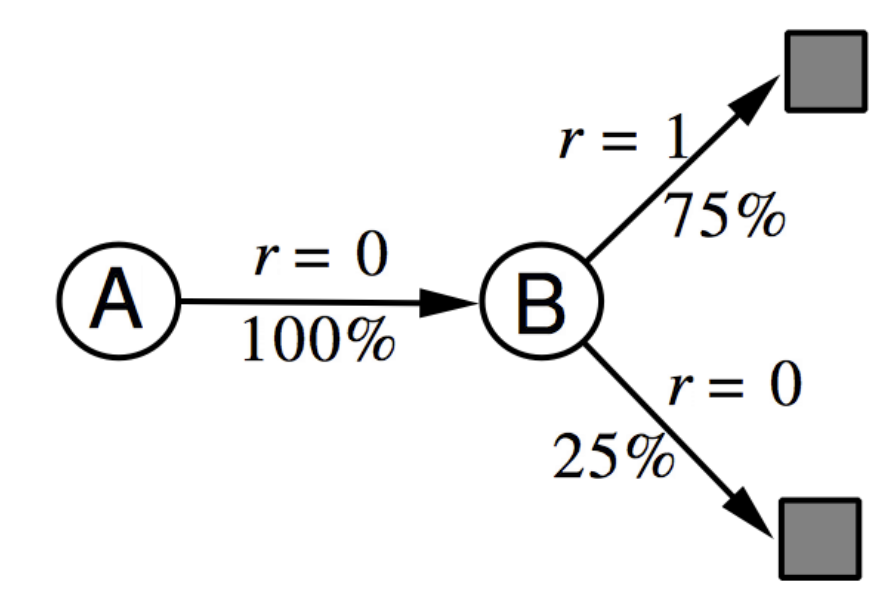
\includegraphics[width=\textwidth]{figures/ab-ex.png}
          \caption{AB Example Revistied}
            \label{fig:ab_ex_1}
        \end{minipage}
      \end{figure}
      And the model is represented the table lookup model as a MDP shown in the \autoref{fig:ab_ex_1}.
\end{example}

\subsubsection{Planning with a Model}
Given a model \(\mathcal{M} _\eta = \langle \mathcal{P}_\eta, \mathcal{R}_\eta \rangle\), we want to solve the 
MDP \(\langle \mathcal{S}, \mathcal{A}, \mathcal{P}_\eta, \mathcal{R}_\eta \rangle\), using any of the 
planning algorithms like dynamic programming, monte carlo tree search, etc.

\subsubsection*{Sample Based Planning}
A simple but powerful approach to a planning. The idea is to use the model only to generate samples:
\[
    \begin{aligned}
        S_{t+1} &\sim \mathcal{P}_\eta(S_{t+1}  | S_t, A_t) \\
        R_{t+1} &= \mathcal{R}_\eta(R_{t+1} | S_t, A_t)
    \end{aligned}        
\]
and then apply model free RL to the samples. Such type of sample-based planning methods are 
often more efficient.


\begin{example}[AB Example]
    Two states \(A\) and \(B\); no discounting; with 8 episodes of experience as:
    \begin{figure}[H]
        \begin{minipage}{0.33\textwidth}
            \[
                \begin{aligned}
                    A, & 0, B, 0 \\
                    B, & 1\\ 
                    B, & 1\\        
                    B, & 1\\        
                    B, & 1\\        
                    B, & 1\\        
                    B, & 1\\        
                    B, & 0\\        
                \end{aligned}
            \]
        \end{minipage}%
        \begin{minipage}{0.33\textwidth}
            % Your first image goes here
            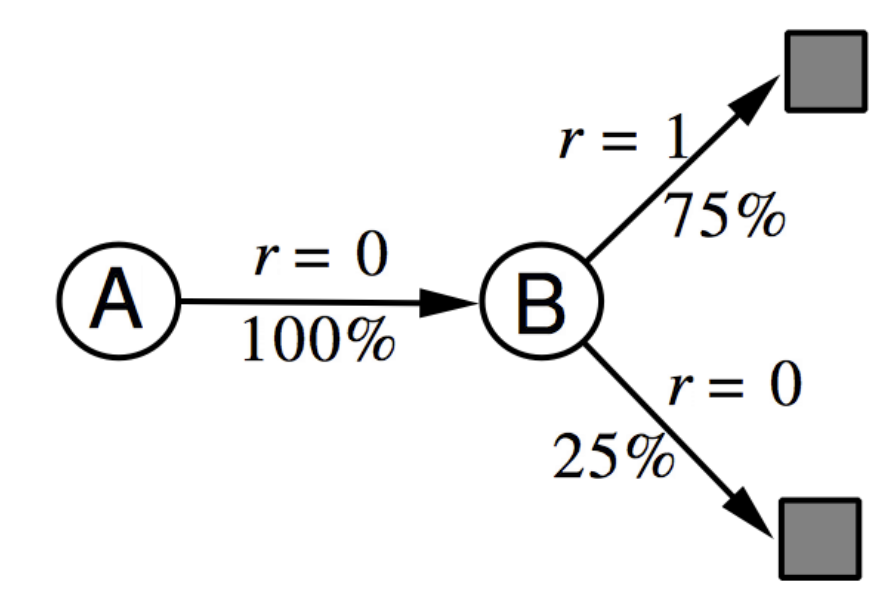
\includegraphics[width=\textwidth]{figures/ab-ex.png}
            \caption{AB Example Revistied}
            \label{fig:ab_ex_2}
        \end{minipage}%
        \begin{minipage}{0.33\textwidth}
            \centering
            Sampled Experience:
            \[
                \begin{aligned}
                    B, & 1\\
                    B, & 0\\
                    B, & 1\\ 
                    A, & 0, B, 0 \\        
                    B, & 1\\        
                    A, & 0, B, 0 \\        
                    B, & 1\\        
                    B, & 0\\ 
                \end{aligned}
            \]
        \end{minipage}
    \end{figure}
    Using Monte Carlo Learning, we can estimate the value function as:
    \[
        \begin{aligned}
            V(A) &= 0 \\
            V(B) &= 0.75\\
        \end{aligned}
    \]
\end{example}

\subsubsection{Planning with an Inaccurate Model}
Given, an imperfect model \(\langle \mathcal{P}_\eta, \mathcal{R}_\eta \rangle \neq \langle \mathcal{P}, \mathcal{R} \rangle\),
then the performance of the model based RL is onlly limited to optimal policy for approximate MDP
\(\langle \mathcal{S}, \mathcal{A}, \mathcal{P}_\eta, \mathcal{R}_\eta \rangle\). i.e. Mopdel based RL is only as good as the model.
So when the model is inacfurate , we will converge to the suboptimal policy. Solutions is to use the model free RL
or to explicitly account for model uncertainty.

\subsection{Integrated Architectures --- Dyna}
We consider two sources of experience.
\begin{itemize}
    \item Sample from enviroment : the tue MDP:
    \[
        \begin{aligned}
            S^{\prime} &\sim \mathcal{P}_{s, s^{\prime}}^{a} \\
            R &=\mathcal{R}_{s, s^{\prime}}^{a}
        \end{aligned}
    \]
    \item Simulated experience: Sampled from model \(\mathcal{M} _\eta\):
    \[
        \begin{aligned}
            S^{\prime} &\sim \mathcal{P}_{\eta}(S^{\prime} | s, a) \\
            R &=\mathcal{R}_{\eta}(R | s, a)
        \end{aligned}  
    \]
\end{itemize}
Thus we have the Dyna architecture which aims to use all the expericence, both real and simulated, to 
learn the value function or the policy. The Dyna architecture is shown in the \autoref{fig:dyna_arch}.
\begin{figure}[H]
    \centering
    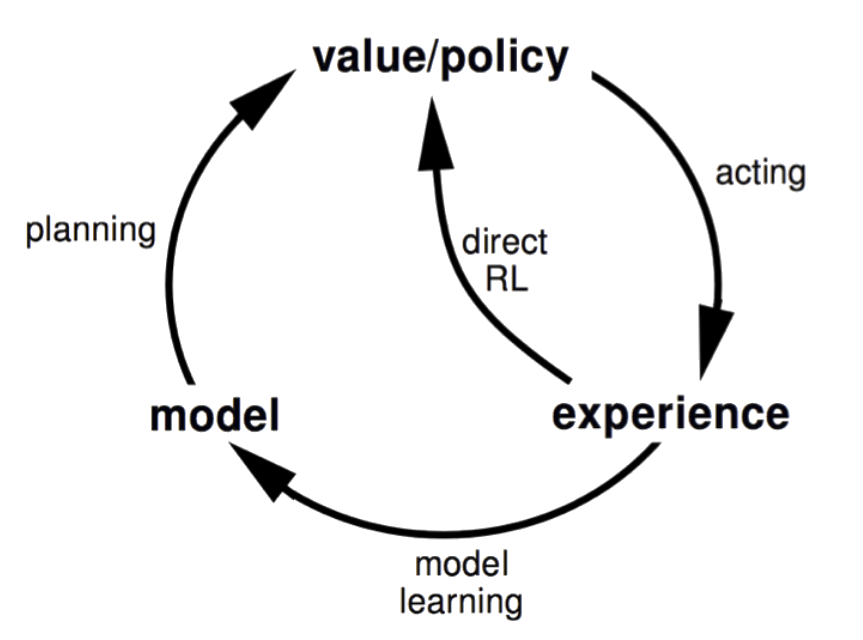
\includegraphics[width=0.5\textwidth]{figures/dyna.png}
    \caption{Dyna Architecture}
    \label{fig:dyna_arch}
\end{figure}

\begin{note}
    lec9 skipped since not required now. Revist later.  
\end{note}